\section{Results}\label{sec:Results}
The selected EBs have orbital periods $2.76- 17.6$ days, with primary masses $0.9 - 2 \mathrm{\ M_{\odot}}$, secondary masses $0.6 - 1.9\ \mathrm{M_{\odot}}$, and effective temperatures $6100- 11000\ \mathrm{K}$. These properties make them suitable as benchmark EBs.\\ 

Shorter orbital periods show evidence of tidal interaction, leading to a potentially circular orbit, confirming theoretical predictions \citep{Justesen21}. EBs of orbital periods $3-8$ days have secondary eclipses occurring at phase 0.5, aligning with this paper. TIC201497357, with an orbital period $< 3$ days, and TIC7695666 and TIC78568736 with periods $> 8$ days required eccentricity parameters to be fitted to minimise residuals. Aligning with \cite{Justesen21}, EBs with extreme separations have higher eccentricities.\\

\citet{Soydugan06} estimated TIC201497357 is located within the instability strip, identifying it as an ALGOL-type EB. The absolute parameters were not determined, so its exact placement within the strip is not confirmed. This Research Note provides the necessary parameters for a reassessment of its potential pulsational variability and classification.\\

Figure \ref{fig:CMD} shows a CMD, identifying the position of the studied EBs. This allows for comparison with the PLATO sample specifications. TIC279087522 has a high mass for both primary and secondary stars ($2\mathrm{M_{\odot}}$ and $1.9\, \mathrm{M_{\odot}}$, respectively). Although the absolute magnitude of the EB ($V \sim 9.88 \mathrm{\ mag}$) is within P1 criteria, the stars are not solar-like and therefore of low priority to PLATO.\\ 

The secondary component of TIC78568736 had a significant error due to the flux contributing $10\%$ and low Gaia coverage at the eclipses, significantly different from the other EBs. However, the primary contribution to the eccentric EB has mass $\sim 1M_{\odot}$ and absolute magnitude $V \sim 10.89\mathrm{\ mag}$ (fulfilling the P1 sample criteria). This primary component is classified as a K-type main-sequence star, suitable for detection and analysis by PLATO. We note TIC279087522 may have underestimated uncertainties due to similarly low Gaia coverage in eclipses (reversing their locations on the CMD).\\

Based on analyses, eight EBs are within the PLATO P1 sample specification, while all ten fulfil the P5 criteria. The EBs have absolute magnitudes $8.4 - 11.5 \mathrm{\ mag}$, and thus all are suitable for detection by PLATO. However, while most are positioned on the main sequence, the required star masses should be $\sim 1 \mathrm{M_{\odot}}$ to be considered a priority target for PLATO \citep{Rauer24}. TIC279087522 and the primary component of TIC201497357 have masses significantly above this ($2\ \mathrm{M_{\odot}}$ and $1.9\ \mathrm{M_{\odot}}$; and $ 1.8\ \mathrm{M_{\odot}}$ respectively), making both systems lower priority targets for PLATO observations.\\


 

\begin{figure}[H]
    \centering
    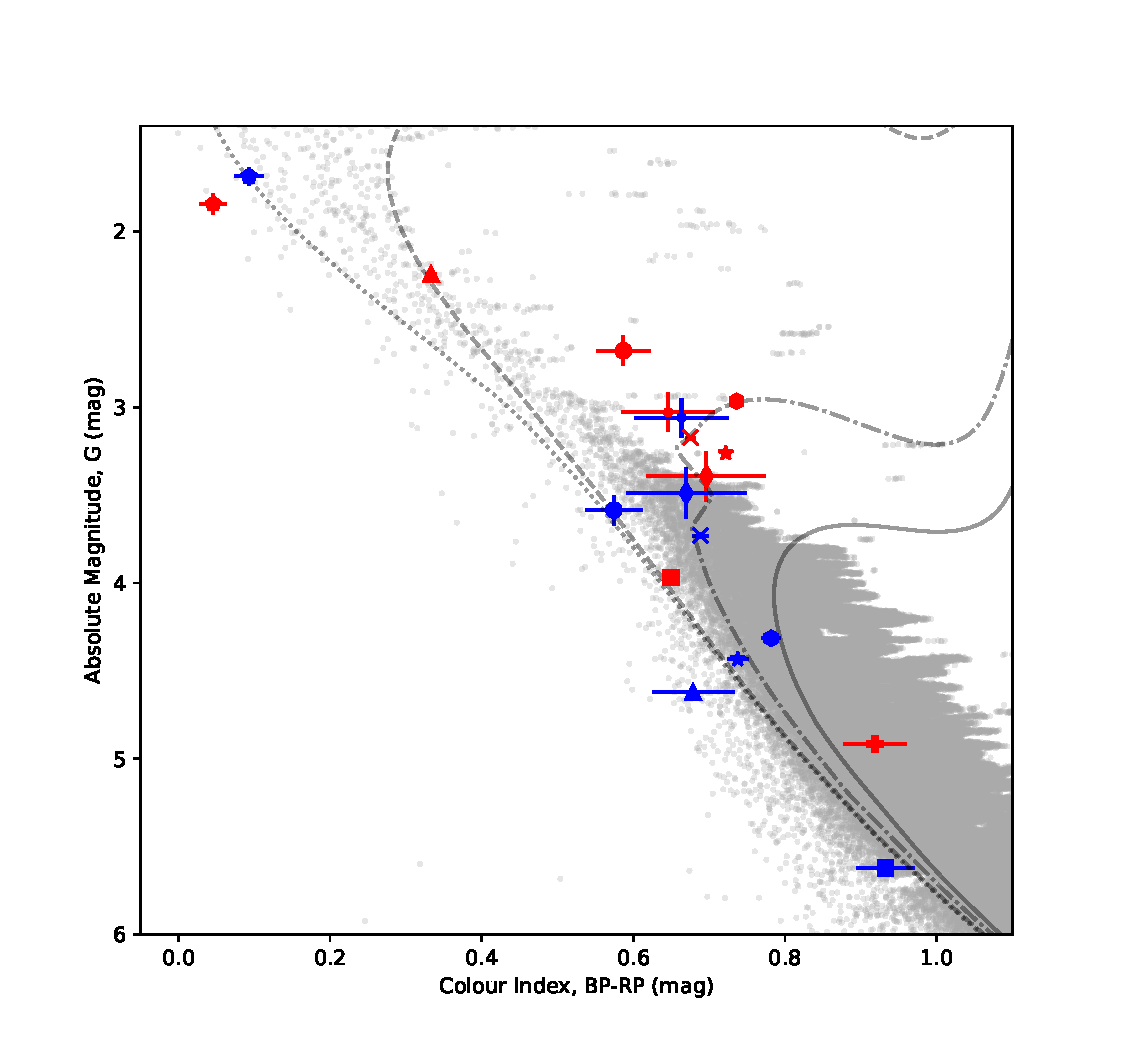
\includegraphics[width=\linewidth]{HRD}
    \caption{The two colours, red and blue, represent primary and secondary components respectively. These symbols represent EBs: TIC279087522 ($\pentagonblack$), TIC30122338 ($\mdblkcircle$), TIC7695666 ($\times$), TIC66602813 ($\mdblksquare$), TIC63579446 ($\bigstar$), TIC201497357 ($\blacktriangle)$, TIC349480507 ($\cdot$), TIC349059354 ($\mdblkdiamond$), TIC78568736 ($+$; secondary outside figure boundaries), TIC80556181 ($\varhexagonblack$). Isochrones from \citet{Dotter16,Choi16,Paxton18} represent stellar ages $0.5 - 10 \mathrm{\ Gyr}$ from left to right. Main sequence stars (grey) are from \citet{Gaia18}}.
    \label{fig:CMD}
\end{figure}